\documentclass[AMA,Times1COL]{WileyNJDv5} %STIX1COL,STIX2COL,STIXSMALL

\articletype{Article Type}%

\received{Date Month Year}
\revised{Date Month Year}
\accepted{Date Month Year}
\journal{Journal}
\volume{00}
\copyyear{2026}
\startpage{1}

\raggedbottom

\begin{document}

\title{GC-EndoGaussian: Residual-Centered Sparse Control for Editable Endoscopic 4D Gaussian Reconstruction}

\author[1]{Mark Taylor}

\author[2,3]{Author Two}

\author[3]{Author Three}

\authormark{TAYLOR \textsc{et al.}}
\titlemark{GC-EndoGaussian: Editable Endoscopic 4D Gaussian Reconstruction}

\address[1]{\orgdiv{Department Name}, \orgname{Institution Name}, \orgaddress{\state{State Name}, \country{Country Name}}}

\address[2]{\orgdiv{Department Name}, \orgname{Institution Name}, \orgaddress{\state{State Name}, \country{Country Name}}}

\address[3]{\orgdiv{Department Name}, \orgname{Institution Name}, \orgaddress{\state{State Name}, \country{Country Name}}}

\corres{Corresponding author Mark Taylor. \email{authorone@gmail.com}}

\presentaddress{Please insert present address text here.}

%\fundingInfo{Text}

\abstract[Abstract]{Dynamic 4D Gaussian Splatting methods can reconstruct deforming tissue from endoscopic video at high visual quality and interactive rendering rates. However, their learned deformation fields provide no explicit handles for manipulating the reconstructed scene after training. This limits their use in applications that require controllable scene deformation, including interactive visualization, augmented-reality overlays, what-if inspection, and surgical training-content generation. We present GC-EndoGaussian, which merges the dense per-Gaussian deformation field of EndoGaussian with the sparse control-node interface of SC-GS to obtain an editable endoscopic 4D reconstruction. The method seeds a sparse set of control nodes over the Gaussian cloud, binds each Gaussian to nearby nodes, predicts time-varying node motion through a graph network, and propagates this motion through a weighted skinning operation. User-specified node translations can then be applied at inference time to produce local edits without retraining: edited tissue follows the commanded handle displacement at a median ratio of 0.96, the induced displacement field is identically zero beyond the binding support of the grabbed nodes, and a new edit re-renders in under 5~ms. Our main contribution is a residual-centered integration recipe that retains near-baseline reconstruction fidelity while adding sparse editing handles: the component that avoids the fidelity loss usually incurred by sparse-control models is a dense per-Gaussian residual, not the graph architecture, which we find interchangeable. At the standard 3000 fine-stage iterations, GC-EndoGaussian is 0.11~dB below EndoGaussian on \texttt{pulling\_soft\_tissues} averaged over four random seeds ($37.07\pm0.06$ vs.\ $37.19\pm0.09$~dB), a gap comparable to seed-to-seed variation; under an extended 6000-iteration schedule, the gap is 0.15~dB on \texttt{pulling\_soft\_tissues} and 0.13~dB on \texttt{cutting\_tissues\_twice}. The method renders at 205~FPS and adds 0.07\% deformation parameters. On SuPer tissue-tracking data, no statistically significant difference from the base model is detected ($p=0.73$). A controlled ablation identifies the per-Gaussian residual as the key component: adding it to an SC-GS-style sparse-control model improves PSNR from $36.80\pm0.01$ to $37.31\pm0.06$~dB across seeds, reduces tracking reprojection error from 7.02 to 3.41 pixels, and repairs a stability failure---without the residual, training diverges on two of five random seeds, whereas every residual-equipped run converges. The residual also confines edits in image space: without it, 40\% of the image change induced by a local edit falls outside the edited region, versus 10--12\% with it.}


\keywords{surgical scene reconstruction, 4D Gaussian Splatting, editable deformation, sparse control nodes, endoscopy}

\jnlcitation{\cname{%
\author{Taylor M.},
\author{Author Two}, and
\author{Author Three}}.
\ctitle{GC-EndoGaussian: Residual-Centered Sparse Control for Editable Endoscopic 4D Gaussian Reconstruction.} \cjournal{\it Journal} \cvol{2026;00(00):1--18}.}

\maketitle

\renewcommand\thefootnote{}
\footnotetext{\textbf{Abbreviations:} 3DGS, 3D Gaussian Splatting; AR, augmented reality; FPS, frames per second; KNN, K-nearest neighbors; PSNR, peak signal-to-noise ratio; RPE, reprojection error.}

\renewcommand\thefootnote{\fnsymbol{footnote}}
\setcounter{footnote}{1}

\section{Introduction}\label{sec1}

Dense reconstruction of deforming tissue from endoscopic video is an important component of computer-assisted intervention. Neural radiance fields and, more recently, 3D Gaussian Splatting (3DGS)~\cite{kerbl2023gaussian} have improved both visual fidelity and rendering speed. Surgical methods including EndoNeRF~\cite{wang2022endonerf}, EndoGaussian~\cite{liu2024endogaussian}, Deform3DGS~\cite{yang2024deform3dgs}, Endo-4DGS, EndoGS, and SurgicalGaussian reconstruct dynamic endoscopic scenes by learning a canonical representation together with a time-dependent deformation field.

These methods are optimized for one thing: \emph{faithfully replaying} the observed deformation. The deformation field is a continuous, per-Gaussian function with no explicit structure and no handles. After training, the motion is fixed---there is no way to ask ``what would this tissue look like if that flap were displaced here?'' Many surgical-vision applications, however, need to \emph{control} the reconstructed scene, not merely replay it: interactive intra-operative visualization, AR overlay and re-planning, what-if inspection of tissue response, and the generation of synthetic-but-plausible training data for downstream models. Concretely, in an augmented-reality guidance overlay a surgeon could displace a tissue flap in the live reconstruction to preview access to an underlying structure; in VR/AR surgical training, an instructor could author varied tissue configurations from a single captured procedure to generate diverse practice scenarios without re-capturing. We present these as \emph{potential applications}---our edits are plausible and produced at negligible cost, not biomechanically validated predictions of tissue response.

Sparse-control methods for dynamic Gaussian scenes provide a natural editing interface. SC-GS~\cite{huang2024scgs}, for example, attaches Gaussians to sparse control points and uses skinning to propagate point motion. Directly replacing a strong endoscopic deformation field with a lower-dimensional sparse-control model, however, can reduce reconstruction fidelity. The central question of this work is therefore:

\begin{quote}
How can sparse editing handles be added to an endoscopic 4D Gaussian reconstruction without discarding the detailed deformation already captured by the base model?
\end{quote}

We address this question with GC-EndoGaussian, which combines sparse node control with a dense per-Gaussian residual. The sparse component provides edit handles, while the residual retains local motion detail that cannot be represented by the shared node field alone. Our contributions are:

\begin{enumerate}[1.]
\item \textbf{A residual-centered integration recipe for editable endoscopic reconstruction.} The final configuration combines translation-only node control, a dense per-Gaussian position residual, fixed nodes, and no coherence regularization. It remains within 0.11~dB of EndoGaussian under the standard training schedule averaged over four random seeds (a gap comparable to seed-to-seed variation) and within 0.15~dB under an extended schedule, while rendering at 205~FPS with 0.07\% additional deformation parameters.

\item \textbf{A sparse edit-control layer for 4D endoscopic Gaussians, evaluated quantitatively.} Motion-seeded control nodes, K-nearest-neighbor soft binding, weighted skinning, and inference-time node translations provide a compact interface for local scene manipulation. We measure the interface directly: handle-following fidelity of $0.96$ (median), structurally compact support (zero displacement beyond the binding neighborhood), foldover rates below $0.14\%$, and sub-5~ms edit-to-render latency. The sparse-control and skinning paradigm follows prior editable Gaussian methods; our contribution is its integration and measurement in a surgical reconstruction pipeline.

\item \textbf{A controlled isolation of the fidelity-preserving component.} A residual-matched comparison shows that an SC-GS-style model without a dense residual loses $0.52$~dB PSNR, has roughly twice the tracking error, leaks $40\%$ of edit-induced image change outside the edited region, and fails to converge on two of five random seeds. The same control architecture with the residual recovers near-baseline reconstruction and tracking, confines edits, and converges on every seed tested.
\end{enumerate}

\section{Related Work}\label{sec2}

\subsection{Dynamic reconstruction for surgery}

EndoNeRF~\cite{wang2022endonerf} introduced neural rendering for deformable tissue reconstruction from stereo endoscopic video. Subsequent 3DGS-based methods~\cite{kerbl2023gaussian} replace volumetric rendering with explicit Gaussian primitives, enabling higher rendering rates. EndoGaussian~\cite{liu2024endogaussian} combines a canonical Gaussian representation with a HexPlane-based~\cite{cao2023hexplane} spatio-temporal deformation field and depth-supervised training. Deform3DGS~\cite{yang2024deform3dgs} introduces learnable Gaussian basis functions to model per-Gaussian tissue deformation with motion-aware point fusion, and further reduces training time relative to HexPlane-style fields. Endo-4DGS~\cite{huang2024endo4dgs} targets the monocular setting, pairing a lightweight MLP deformation field with Depth-Anything pseudo-depth priors for initialization. EndoGS~\cite{zhu2024endogs} reconstructs deformable tissue from single-viewpoint video using depth-guided spatiotemporal weight masks and surface-aligned regularization, while SurgicalGaussian~\cite{xie2024surgicalgaussian} models soft-tissue dynamics with a forward-mapping deformation MLP regularized to keep neighboring Gaussians moving consistently. EndoGSLAM~\cite{wang2024endogslam} and Free-SurGS~\cite{guo2024freesurgs} instead target simultaneous localization and mapping, performing dense Gaussian reconstruction jointly with camera-pose estimation in settings where Structure-from-Motion is unreliable on textureless tissue. LGS~\cite{liu2024lgs} and HFGS~\cite{zhao2024hfgs} pursue lightweight and high-frequency-aware deformation representations, respectively, while EndoSparse~\cite{li2024endosparse} addresses sparse-view endoscopic capture. These methods emphasize reconstruction fidelity and rendering efficiency, but do not expose sparse handles for post-training scene manipulation.

\subsection{General dynamic and deformable Gaussian Splatting}

Beyond the surgical domain, several methods extend 3DGS~\cite{kerbl2023gaussian} to dynamic scenes using a canonical-Gaussian-plus-deformation-field paradigm. Deformable 3D Gaussians~\cite{yang2024deformable3dgaussians} learns an MLP deformation field over a canonical Gaussian set for monocular dynamic scene reconstruction, and 4D Gaussian Splatting~\cite{wu2024fourdgs} uses a HexPlane-style~\cite{cao2023hexplane} decomposed neural-voxel encoding with a lightweight decoder to predict Gaussian deformation at arbitrary timestamps; this is the architectural family that EndoGaussian~\cite{liu2024endogaussian} adapts to endoscopy. Dynamic 3D Gaussians~\cite{luiten2024dynamic3dgaussians} instead tracks persistent Gaussians over time under local-rigidity constraints, foreshadowing the local-rigidity priors used by sparse-control editing methods. GaussianFlow~\cite{gao2024gaussianflow} supervises Gaussian dynamics with 2D optical flow, and PhysGaussian~\cite{xie2024physgaussian} replaces the learned deformation field entirely with a physics simulator (the Material Point Method) acting on each Gaussian as a continuum particle, offering a physically grounded alternative to learned deformation. Closest to our setting, SC-GS~\cite{huang2024scgs} represents a dynamic scene with a sparse set of control points and propagates their motion to dense Gaussians via K-nearest-neighbor skinning, enabling editing by manipulating a small number of control handles; CoGS~\cite{yu2024cogs} similarly supports direct, real-time manipulation of dynamic scene elements without precomputed control signals. GC-EndoGaussian adopts the sparse-control-and-skinning paradigm established by SC-GS, but integrates it with a dense per-Gaussian residual to preserve the fine-grained deformation fidelity that a purely sparse graph cannot represent, and evaluates it in the deformable-tissue setting.

\subsection{Editable neural radiance fields and Gaussian scenes}

Editability has also been explored for implicit neural representations. NeRF-Editing~\cite{yuan2022nerfediting} extracts an explicit mesh proxy from a trained NeRF and applies established mesh-deformation tools (e.g., as-rigid-as-possible warping) before bending camera rays through a tetrahedral cage, while CoNeRF~\cite{kania2022conerf} treats semantic attributes as latent variables regressed from sparse, mask-annotated supervision to enable controllable rendering. EditableNeRF~\cite{zheng2023editablenerf} automatically discovers sparse key points on a topologically varying dynamic NeRF and lets users drag them to edit the scene, which is the closest neural-field precedent to our node-based control interface. Instruct-NeRF2NeRF~\cite{haque2023instructnerf2nerf} instead edits a reconstructed scene from natural-language instructions via an image-conditioned diffusion model, representing a generative and semantic editing paradigm rather than an explicit geometric one. Within the Gaussian Splatting literature, GaussianEditor~\cite{chen2024gaussianeditor} performs swift, controllable 3D editing using Gaussian semantic tracing and hierarchical Gaussian representations. Unlike these general-purpose or semantic editing approaches, GC-EndoGaussian targets explicit, local, drag-based control of a reconstructed deformable-tissue scene at inference time, without retraining or text-conditioned generation.

\subsection{Skinning and deformation-graph representations}

Sparse-control editing of Gaussians builds on a long line of work in mesh and skeletal deformation. Linear blend skinning, in which surface points are expressed as weighted combinations of transformations at a sparse set of handles, originates with the joint-dependent local deformation model of Magnenat-Thalmann et al.~\cite{magnenatthalmann1988jld} and was later refined by pose-space deformation~\cite{lewis2000posespace} to reduce classical skinning artifacts. Deformation transfer~\cite{sumner2004deformationtransfer} propagates per-triangle transformations from a source deformation onto a target mesh, and embedded deformation graphs~\cite{sumner2007embedded} generalize this idea by defining a space deformation from a sparse graph of affine transformations blended smoothly over nearby geometry---the model that our control-node-and-skinning formulation, and SC-GS-style representations more broadly, directly generalize to dynamic Gaussians. As-rigid-as-possible surface modeling~\cite{sorkine2007arap} formalizes a local-rigidity energy that penalizes non-rigid distortion during deformation, motivating the coherence regularizers commonly paired with sparse control; we find in our ablations (Section~\ref{sec:residual}) that such priors are not necessary once a dense per-Gaussian residual is present. Finally, dual quaternion skinning~\cite{kavan2007dualquaternion,kavan2008geometricskinning} blends rigid transformations in a way that avoids the volume-collapsing artifacts of linear blend skinning, motivating our choice to restrict the general control formulation's rotation component when translation-only control is sufficient for the endoscopic setting.

\section{Method}\label{sec3}

\subsection{Base 4D Gaussian reconstruction}

The reconstructed scene contains approximately $N\approx30\text{k}$ canonical 3D Gaussians. Gaussian $i$ has canonical position $x_i$, rotation, scale, opacity, and spherical-harmonic color coefficients. At timestamp $t$, a HexPlane-style~\cite{cao2023hexplane} spatio-temporal field produces a feature for each Gaussian. Small prediction heads then output changes in position, rotation, scale, and opacity.

Training follows the two-stage procedure of the base method. A coarse stage estimates static geometry, and a fine stage activates the dynamic deformation model. Supervision includes a tool-masked photometric loss, an inverse-depth loss in binocular mode, and total-variation regularization on the spatio-temporal field.

This dense deformation model provides high reconstruction quality but no explicit post-training control handles.

\subsection{Sparse control-node graph}

At the beginning of the fine stage, we initialize $M=1024$--$2048$ control nodes over the Gaussian cloud. Nodes are selected using motion-weighted farthest-point sampling. Farthest-point sampling encourages spatial coverage, while accumulated deformation magnitude gives greater sampling weight to regions exhibiting stronger motion.

Each Gaussian is bound to its $K=4$ nearest nodes. For Gaussian $i$ and neighboring node $k$, the normalized binding weight is
\begin{equation}\label{eq:weight}
w_{ik}=\frac{\exp\!\left(-\lVert x_i-n_k\rVert^2/\sigma^2\right)}
{\sum_{j\in\mathcal N(i)}\exp\!\left(-\lVert x_i-n_j\rVert^2/\sigma^2\right)},
\end{equation}
where $n_k$ is the canonical position of node $k$ and $\mathcal N(i)$ is the set of nodes bound to Gaussian $i$. Bindings are rebuilt when densification changes the Gaussian set. In the final configuration, node positions are fixed after initialization.

\begin{figure}[t]
\centering
\includegraphics[width=0.8\columnwidth]{figures/pipeline_horizontal.png}
\caption{GC-EndoGaussian adds a sparse control path to the dense deformation model. The final configuration blends node translations and then adds a dense per-Gaussian residual. Rotation, scale, and opacity remain controlled by the base deformation field.\label{fig:pipeline}}
\end{figure}



\subsection{Node-motion network}

For each node $k$ and timestamp $t$, an MLP first encodes the node position and time:
\begin{equation}\label{eq:nodeenc}
h_k^0=\mathrm{MLP}\!\left([\gamma(n_k),\gamma(t)]\right),
\end{equation}
where $\gamma$ denotes positional encoding. The default implementation applies two EdgeConv-style~\cite{wang2019dgcnn} message-passing layers over a K-nearest-neighbor node graph before predicting node motion.

The general implementation can output a rigid transformation $(R_k,t_k)$. This full $SE(3)$ form is used for the SC-GS-style comparison and related ablations. For all results labeled \textbf{ours (match)}, node rotation is disabled by setting $R_k=I$, and the graph predicts translation only. This distinction avoids ambiguity between the general control implementation and the final model evaluated in the main tables.

The output layer is initialized to zero translation, making the control path an initial no-op. Node identity is encoded through node position rather than through a learned node-specific embedding.

Message passing is not essential to the main result. A node-wise MLP without graph layers performs similarly in the residual-matched ablation, indicating that the dense residual, rather than the graph aggregator, is responsible for retaining fidelity.

\subsection{Weighted deformation and edit handle}

For the general $SE(3)$ control formulation, Gaussian position can be warped by linear blend skinning:
\begin{equation}\label{eq:skin}
p_i^{\mathrm{node}}(t)=\sum_{k\in\mathcal N(i)}w_{ik}
\left[R_k(t)(x_i-n_k)+n_k+t_k(t)\right].
\end{equation}
In the final translation-only configuration, $R_k=I$, and this simplifies to a weighted translation field. Let $r_i(t)$ denote the dense per-Gaussian position residual predicted from the base spatio-temporal feature. The final Gaussian position is
\begin{equation}\label{eq:final}
p_i(t)=x_i+\sum_{k\in\mathcal N(i)}w_{ik}\,t_k(t)+r_i(t).
\end{equation}
Gaussian rotation, scale, and opacity are predicted by the corresponding heads of the base deformation model and are not blended from control-node rotations in the final configuration.

At inference time, a user-provided translation $e_k$ can be assigned to one or more nodes. The edited position becomes
\begin{equation}\label{eq:edit}
p_i^{\mathrm{edit}}(t)=p_i(t)+\sum_{k\in\mathcal N(i)}w_{ik}\,e_k.
\end{equation}
This produces a local, smoothly weighted edit without retraining. With approximately 2048 nodes controlling approximately 30,000 Gaussians, the representation provides a control ratio of roughly 15:1. Non-finite deformation outputs are replaced by the corresponding unmodified values before rasterization.

\begin{figure}[t]
\centering
\begin{minipage}[t]{0.32\columnwidth}\centering
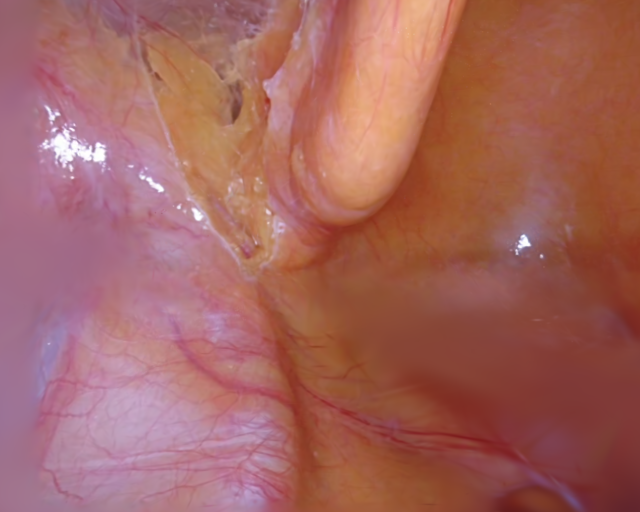
\includegraphics[width=\linewidth,height=100pt]{figures/edit_before.png}\\[2pt]{\footnotesize before}
\end{minipage}\hfill
\begin{minipage}[t]{0.32\columnwidth}\centering
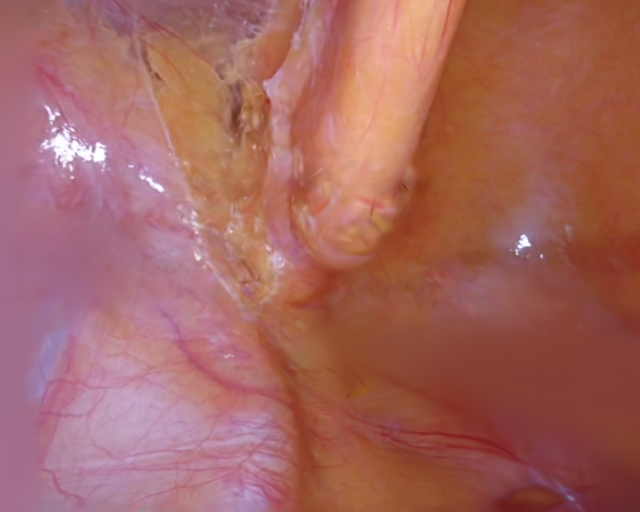
\includegraphics[width=\linewidth,height=100pt]{figures/edit_after.png}\\[2pt]{\footnotesize after}
\end{minipage}\hfill
\begin{minipage}[t]{0.32\columnwidth}\centering
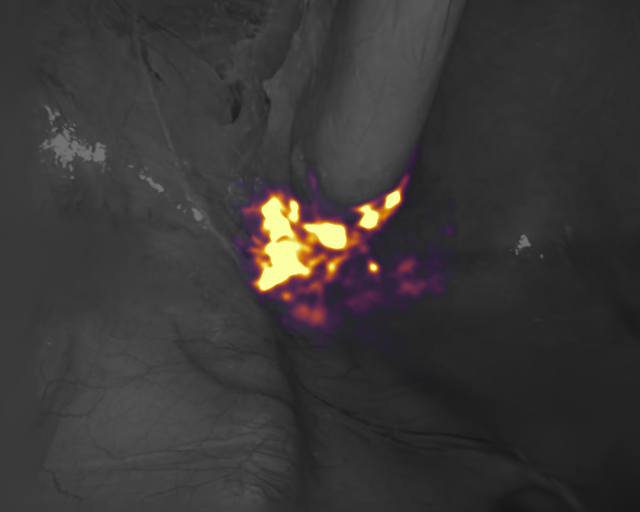
\includegraphics[width=\linewidth,height=100pt]{figures/edit_diff.png}\\[2pt]{\footnotesize diff}
\end{minipage}
\caption{Qualitative drag-to-edit example. Left: reconstruction before editing. Middle: reconstruction after translating a local group of control nodes. Right: per-pixel edit-magnitude visualization. The example illustrates the locality of the weighted control operation; it does not establish biomechanical validity.\label{fig:edit}}
\end{figure}

\begin{figure}[t]
\centering
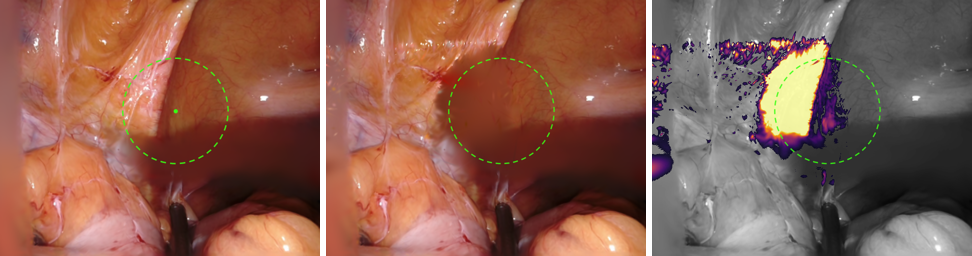
\includegraphics[width=\columnwidth,height=100pt]{figures/edit_reveal_cutting_preview.png}
\caption{Editable tissue retraction on \texttt{cutting\_tissues\_twice}. A local group
of control nodes (dashed outline) is dragged laterally at inference time to retract the
overlying tissue and expose the region behind it, without retraining. Left: before;
middle: after lateral retraction; right: per-pixel edit magnitude
$\lVert I_{\mathrm{after}}-I_{\mathrm{before}}\rVert$, localized to the retracted
region. The edit illustrates controllable visibility; it does not model tissue mechanics
or establish biomechanical validity.\label{fig:edit_reveal}}
\end{figure}


\subsection{Residual-centered integration recipe}

A sparse control graph that replaces the dense deformation field loses reconstruction detail. The final \textbf{match} configuration therefore uses four design choices:

\begin{itemize}
\item \textbf{Translation-only node control.} The sparse graph controls Gaussian position only. Rotation, scale, and opacity remain under the dense base deformation model.
\item \textbf{Dense per-Gaussian position residual.} A residual head evaluated for each Gaussian restores local motion detail that cannot be represented by a low-dimensional shared node field.
\item \textbf{No ARAP, isometric, or temporal coherence loss.} These priors can bias highly non-rigid tissue motion away from the photometric optimum.
\item \textbf{Fixed control nodes.} Nodes are not re-seeded after initialization, avoiding optimization disruptions caused by changes in the control representation.
\end{itemize}

The residual-matched study in Section~\ref{sec:residual} shows that the per-Gaussian residual is the dominant component. The remaining choices simplify optimization and avoid unnecessary constraints, but do not independently explain the full fidelity recovery.

\section{Experiments}\label{sec4}

\subsection{Datasets}

We evaluate reconstruction on the EndoNeRF~\cite{wang2022endonerf} \texttt{pulling\_soft\_tissues} sequence with 63 frames and \texttt{cutting\_tissues\_twice} with 156 frames. Both are processed in binocular mode at $640\times512$ resolution, with every eighth frame held out for testing.

Tracking is evaluated on four SuPer~\cite{li2020super} trials containing da Vinci tissue-manipulation sequences. Each trial contains 26--51 manually annotated tissue points over 151 frames. The data are converted to the reconstruction pipeline using stereo-SGBM depth, tool masks, and static-camera poses. The primary tracking comparison aggregates the four trials. The residual-isolation ablation reports SuPer trial 3, as stated in its table.

\subsection{Baselines}

We compare against:
\begin{itemize}
\item \textbf{EndoGaussian:} the dense base model without sparse editing controls.
\item \textbf{SC-GS-style control:} an implementation of independent sparse control points with full $SE(3)$ motion, ARAP regularization, adaptive re-seeding, no graph message passing, and 2048 control points.
\item \textbf{SC-GS-style + residual:} the same sparse-control architecture augmented with the dense per-Gaussian residual used in GC-EndoGaussian.
\end{itemize}

The SC-GS-style models are implemented and trained inside the same reconstruction pipeline to reduce differences unrelated to the deformation representation.

\subsection{Metrics and implementation}

Reconstruction quality is measured using PSNR, SSIM, LPIPS, and depth RMSE on held-out frames. Tracking is measured as 2D reprojection error against the SuPer annotations. We report bootstrap 95\% confidence intervals for the primary tracking comparison and use a paired Wilcoxon signed-rank test.

Efficiency is measured using rendering speed, deformation-parameter count, and edit-to-render latency. Training schedules are compared by optimization-step count; wall-clock training-time measurements are not reported.

Experiments use one NVIDIA H100 GPU with PyTorch 2.5.1, CUDA 12.x, and Python 3.12. Unless stated otherwise, GC-EndoGaussian uses 2048 control nodes, four node bindings per Gaussian, and two graph layers. The standard schedule contains 1000 coarse-stage and 3000 fine-stage iterations. The extended comparison increases the fine stage to 6000 iterations for both methods.

Reconstruction robustness to initialization is reported as mean $\pm$ standard deviation over four random seeds per configuration on \texttt{pulling\_soft\_tissues} under the standard schedule (Table~\ref{tab:seeds}). Editing is evaluated with five interface metrics (Section~\ref{sec:edit_eval}): \emph{handle fidelity} (achieved displacement of strongly-bound Gaussians divided by the commanded magnitude), \emph{3D leakage} (mean normalized displacement of Gaussians beyond twice the handle radius), \emph{pixel leakage} (fraction of image change outside the dilated projected footprint of the edited region), \emph{foldover rate} (fraction of Gaussian $k$-NN pairs whose relative orientation inverts under the edit), and \emph{edit latency} (wall-clock from setting a new edit vector to a completed $640\times512$ re-render). Each edit metric aggregates 32 edits: 8 handle draws $\times$ 4 magnitudes (1--8\% of scene extent), with handle radius $0.10\times$ the scene extent.

\section{Results}\label{sec5}

\subsection{Reconstruction remains close to the dense baseline}

Table~\ref{tab:recon} compares GC-EndoGaussian with EndoGaussian under the standard and extended training schedules. Under the standard 3000-iteration fine stage on \texttt{pulling\_soft\_tissues}, the editable model is 0.11~dB lower in PSNR averaged over four random seeds (Table~\ref{tab:seeds}); per-configuration seed variation is $\leq 0.09$~dB, so the single-seed gaps in Table~\ref{tab:recon} should be read with that granularity in mind. Under the extended schedule, the difference is 0.15~dB on \texttt{pulling\_soft\_tissues} and 0.13~dB on \texttt{cutting\_tissues\_twice}. SSIM, LPIPS, and depth RMSE also remain close but consistently favor the dense baseline in these comparisons.

\begin{table*}[t]%
\centering
\caption{Reconstruction under matched optimization schedules. $\Delta$PSNR is GC-EndoGaussian minus EndoGaussian.\label{tab:recon}}%
\begin{tabular*}{\textwidth}{@{\extracolsep\fill}lllccccc@{\extracolsep\fill}}
\toprule
\textbf{Dataset} & \textbf{Fine-stage} & \textbf{Method} & \textbf{PSNR}$\uparrow$ & \textbf{SSIM}$\uparrow$ & \textbf{LPIPS}$\downarrow$ & \textbf{Depth-RMSE}$\downarrow$ & \textbf{$\Delta$PSNR} \\
\midrule
pulling & 3000 & EndoGaussian     & 37.27 & 0.9578 & 0.0609 & 2.906 & --- \\
pulling & 3000 & GC-EndoGaussian  & 37.00 & 0.9559 & 0.0638 & 3.139 & $-0.27$ \\
pulling & 6000 & EndoGaussian     & 37.32 & 0.9578 & 0.0509 & 2.646 & --- \\
pulling & 6000 & GC-EndoGaussian  & 37.17 & 0.9567 & 0.0533 & 2.793 & $-0.15$ \\
cutting & 6000 & EndoGaussian     & 39.42 & 0.9696 & 0.0322 & 1.358 & --- \\
cutting & 6000 & GC-EndoGaussian  & 39.29 & 0.9689 & 0.0339 & 1.384 & $-0.13$ \\
\bottomrule
\end{tabular*}
\end{table*}

These results do not demonstrate numerical equivalence. They show that adding sparse control produces a small, measurable reconstruction cost while retaining performance close to the dense baseline.

\begin{table}[t]%
\centering
\caption{Seed robustness on \texttt{pulling\_soft\_tissues} (standard schedule). Mean $\pm$ standard deviation over four converged seeds per configuration. The residual-free SC-GS-style model additionally \emph{failed to converge on two of five attempted seeds} (one collapse to 7.5~dB, one reproducible CUDA failure during node-graph training); no residual-equipped configuration failed on any seed.\label{tab:seeds}}%
\begin{tabular*}{\columnwidth}{@{\extracolsep\fill}lccc@{\extracolsep\fill}}
\toprule
\textbf{Method} & \textbf{PSNR}$\uparrow$ & \textbf{LPIPS}$\downarrow$ & \textbf{Converged} \\
\midrule
EndoGaussian             & $37.19 \pm 0.09$ & $0.062 \pm 0.001$ & 4/4 \\
SC-GS-style, no residual & $36.80 \pm 0.01$ & $0.090 \pm 0.001$ & 3/5 \\
SC-GS-style + residual   & $37.31 \pm 0.06$ & $0.065 \pm 0.000$ & 4/4 \\
GC-EndoGaussian          & $37.07 \pm 0.06$ & $0.065 \pm 0.001$ & 4/4 \\
\bottomrule
\end{tabular*}
\end{table}

\begin{figure*}[t]
\centerline{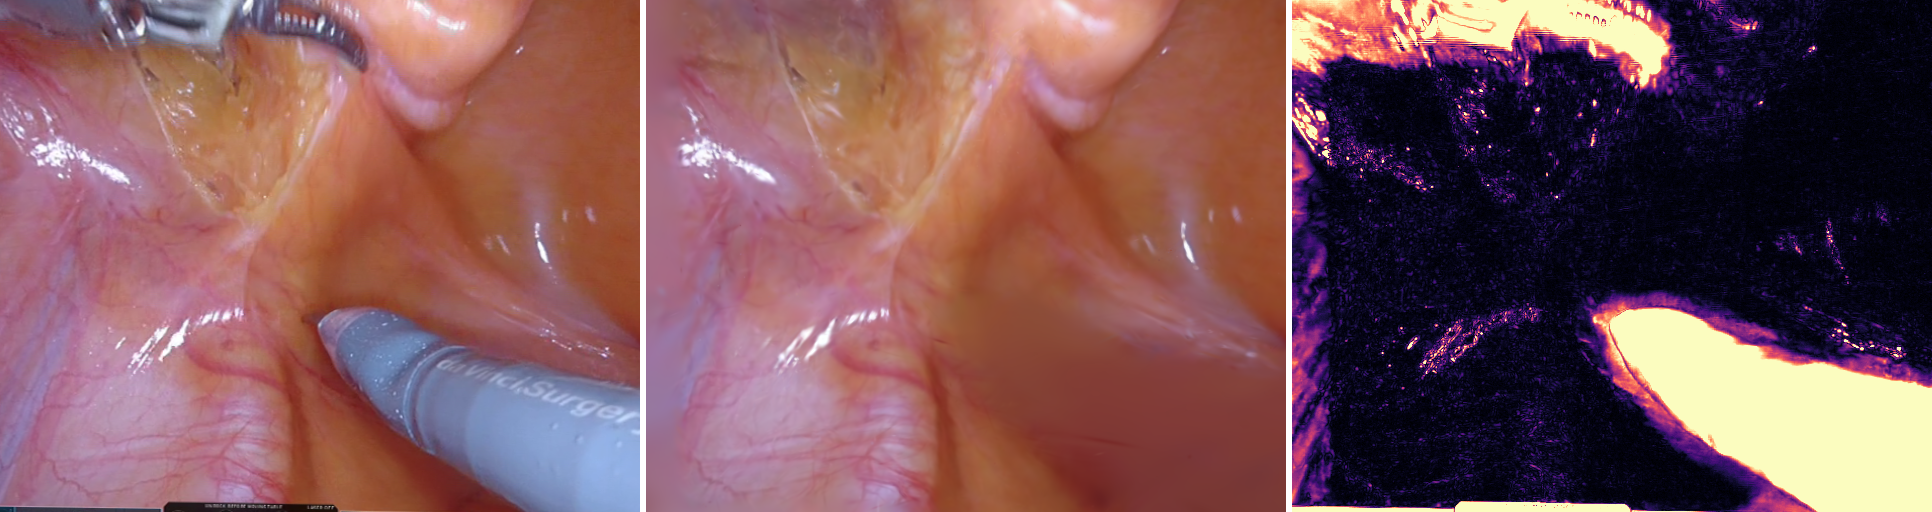
\includegraphics[width=\textwidth,height=8pc]{figures/recon_pulling_triptych.png}}
\caption{Reconstruction on \texttt{pulling\_soft\_tissues}, frame 40. Left: ground truth. Center: GC-EndoGaussian rendering. Right: per-pixel error map. The visualization complements the aggregate metrics in Table~\ref{tab:recon}.\label{fig:recon}}
\end{figure*}

\subsection{Runtime and parameter overhead}

GC-EndoGaussian remains suitable for interactive rendering. The sparse control path reduces rendering speed from 285 to 205~FPS but remains well above real-time rates. It increases the deformation-model parameter count from 85.29~M to 85.35~M, corresponding to 0.07\% additional parameters. Applying a new edit vector and re-rendering one $640\times512$ frame takes 4.8~ms (median), so the edit loop itself also runs at interactive rates.

\begin{table}[t]%
\centering
\caption{Efficiency on \texttt{pulling\_soft\_tissues}.\label{tab:eff}}%
\begin{tabular*}{\columnwidth}{@{\extracolsep\fill}lcc@{\extracolsep\fill}}
\toprule
\textbf{Metric} & \textbf{EndoGaussian} & \textbf{GC-EndoGaussian} \\
\midrule
Render speed             & 285 FPS               & 205 FPS \\
Edit-to-render latency   & ---                   & 4.8 ms \\
Deformation parameters   & 85.29 M               & 85.35 M \\
Parameter increase       & ---                   & $+0.07\%$ \\
Optimization schedule    & $1000+3000$           & $1000+3000$ \\
\bottomrule
\end{tabular*}
\end{table}

The table compares optimization-step counts rather than wall-clock training time. The additional graph and blending operations increase per-iteration computation, so unchanged iteration count should not be interpreted as unchanged training duration.

\subsection{Quantitative edit evaluation}\label{sec:edit_eval}

Table~\ref{tab:edit} measures the editing interface directly on the three budget-matched models of Table~\ref{tab:residual}. All models follow the handle at a median fidelity of $0.96$--$0.97$, with \emph{identically zero} displacement beyond the binding support of the grabbed nodes (Figure~\ref{fig:locality})---locality is a structural property of the compact K-nearest-neighbor binding, independent of training. Foldover rates remain below $0.14\%$ of Gaussian neighbor pairs at all tested magnitudes, and a new edit re-renders in under $5$~ms, so the edit loop runs at interactive rates on top of the 205~FPS renderer.

The models differ sharply in \emph{pixel-space} hygiene: without the dense residual, $40\%$ of the total image change induced by a local edit falls outside the edited region's footprint, versus $10$--$12\%$ for the residual-equipped models. The residual absorbs appearance detail that the sparse graph would otherwise distribute globally, so removing it does not only cost reconstruction fidelity (Table~\ref{tab:residual})---it also makes edits visually leak. Finally, decomposing the learned motion of the hybrid models shows the node field carries $23$--$31\%$ of the deformation energy and the residual the remaining $69$--$77\%$: the sparse graph is an \emph{interface} over a predominantly dense motion model, consistent with Section~\ref{sec:residual}.

\begin{table}[t]%
\centering
\caption{Edit-interface metrics on \texttt{pulling\_soft\_tissues} (3000 fine-stage iterations, matched budget). Median over 32 edits (8 handle draws $\times$ 4 magnitudes, 1--8\% of scene extent). Fid.\ = handle fidelity; L\textsubscript{3D} = normalized displacement beyond $2\times$ handle radius; L\textsubscript{px} = image change outside the edited footprint; Fold = foldover rate; Lat.\ = edit-to-render latency; R.\,frac.\ = fraction of learned motion energy carried by the dense residual.\label{tab:edit}}%
\begin{tabular*}{\columnwidth}{@{\extracolsep\fill}lcccccc@{\extracolsep\fill}}
\toprule
\textbf{Method} & \textbf{Fid.}$\uparrow$ & \textbf{L\textsubscript{3D}}$\downarrow$ & \textbf{L\textsubscript{px}}$\downarrow$ & \textbf{Fold}$\downarrow$ & \textbf{Lat.}$\downarrow$ & \textbf{R.\,frac.} \\
\midrule
SC-GS-style, no residual & 0.97 & 0.0\% & 40.4\% & 0.07\% & 4.5 ms & --- \\
SC-GS-style + residual   & 0.97 & 0.0\% & \phantom{0}9.6\% & 0.08\% & 4.7 ms & 0.69 \\
GC-EndoGaussian          & 0.96 & 0.0\% & 12.3\% & 0.05\% & 4.8 ms & 0.77 \\
\bottomrule
\end{tabular*}
\end{table}

\begin{figure}[t]
\centering
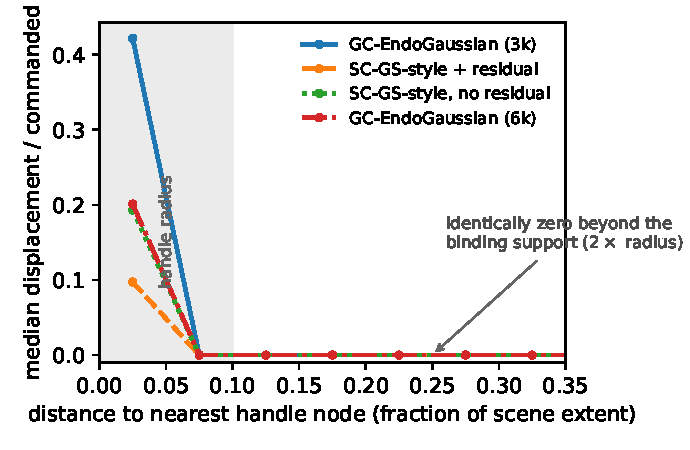
\includegraphics[width=0.9\linewidth]{figures/fig_edit_locality.pdf}
\caption{Edit locality. Median per-Gaussian displacement (normalized by the commanded magnitude) as a function of distance to the nearest grabbed control node, aggregated over 32 edits. The displacement field falls off within the handle radius (shaded) and is identically zero beyond the K-nearest-neighbor binding support---locality is structural, not learned.\label{fig:locality}}
\end{figure}

\subsection{Tracking shows no detected difference from EndoGaussian}

Across the four SuPer trials, median reprojection error is 3.30 pixels for GC-EndoGaussian and 3.47 pixels for EndoGaussian. The corresponding bootstrap 95\% confidence intervals are $[3.14, 3.46]$ and $[3.34, 3.59]$. A paired Wilcoxon signed-rank test gives $p=0.73$.

The appropriate interpretation is that the experiment detects no statistically significant difference in tracking error between the two models. This result is not an equivalence test and should not be interpreted as proof that the methods are identical within a predefined margin; with four trials, the paired test also has minimal statistical power (the smallest attainable two-sided $p$ at $n{=}4$ is $0.125$).

The residual-free SC-GS-style model provides a more informative contrast. On SuPer trial 3, its median reprojection error is 7.02 pixels. Adding the dense residual reduces this error to 3.41 pixels, close to GC-EndoGaussian at 3.30 pixels and EndoGaussian at 3.47 pixels.

\begin{figure*}[t]
\centerline{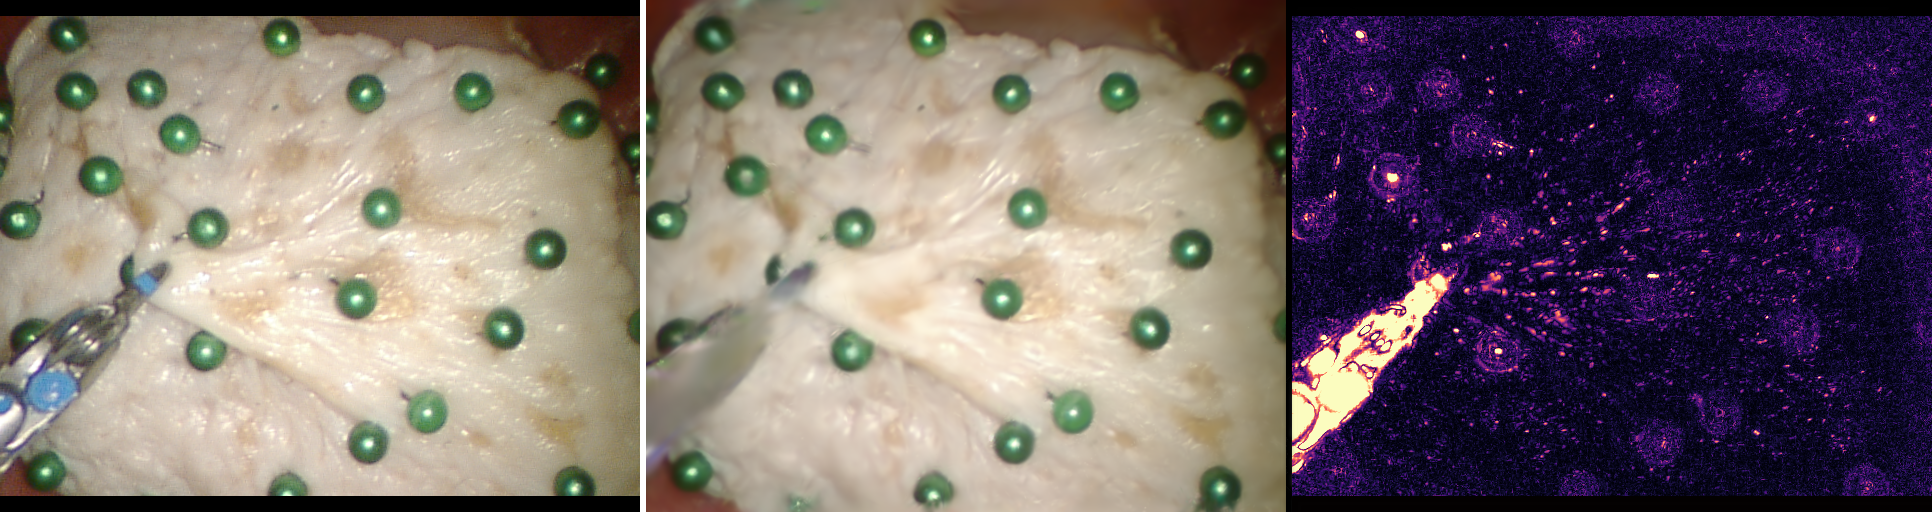
\includegraphics[width=\textwidth,height=10pc]{figures/recon_super_t3_triptych2.png}}
\caption{Reconstruction on SuPer trial 3, frame 90. Left: ground truth. Center: GC-EndoGaussian rendering. Right: per-pixel error visualization. Discs indicate annotated tissue points used in tracking evaluation.\label{fig:super}}
\end{figure*}

\subsection{The dense residual is the key fidelity-preserving component}\label{sec:residual}

Which part of the recipe keeps editing reconstruction-neutral---the graph message passing, the translation-only design, or the per-Gaussian residual? Table~\ref{tab:residual} answers cleanly: we train an SC-GS-style control with and without the per-Gaussian residual, at the same 3000-iteration budget, and compare to GC-EndoGaussian. The residual-free model achieves 36.80~dB and 7.02-pixel tracking error. Adding the residual raises PSNR to 37.29~dB and lowers tracking error to 3.41 pixels---recovering the entire gap. This recovery occurs without adopting GC-EndoGaussian's graph message passing or translation-only control. Across seeds, the recovery is $0.52$~dB ($36.80\pm0.01$ to $37.31\pm0.06$; Table~\ref{tab:seeds}), roughly six times the per-configuration seed variation.

Two further observations sharpen this conclusion. First, the residual-free model is not merely worse but \emph{unstable}: across five random seeds it diverged twice (one collapse to 7.5~dB, one reproducible failure during node-graph optimization), whereas every residual-equipped configuration converged on all four seeds tested (Table~\ref{tab:seeds}). Second, the gap is visible: Figure~\ref{fig:residual_visual} shows the residual-free model smearing high-frequency vascular texture and specular highlights that the dense residual restores without changing the control architecture.

\begin{table}[t]%
\centering
\caption{Residual isolation. Reconstruction is reported on \texttt{pulling\_soft\_tissues} after 3000 fine-stage iterations. Tracking is median reprojection error on SuPer trial 3.\label{tab:residual}}%
\begin{tabular*}{\columnwidth}{@{\extracolsep\fill}lcccc@{\extracolsep\fill}}
\toprule
\textbf{Method} & \textbf{PSNR}$\uparrow$ & \textbf{SSIM}$\uparrow$ & \textbf{LPIPS}$\downarrow$ & \textbf{Track RPE}$\downarrow$ \\
\midrule
EndoGaussian, no editing & 37.27 & 0.9578 & 0.0609 & 3.47 \\
SC-GS-style, no residual & 36.80 & 0.9505 & 0.0885 & 7.02 \\
SC-GS-style + residual   & 37.29 & 0.9570 & 0.0649 & 3.41 \\
GC-EndoGaussian          & 37.00 & 0.9559 & 0.0638 & 3.30 \\
\bottomrule
\end{tabular*}
\end{table}

\begin{figure*}[t]
\centering
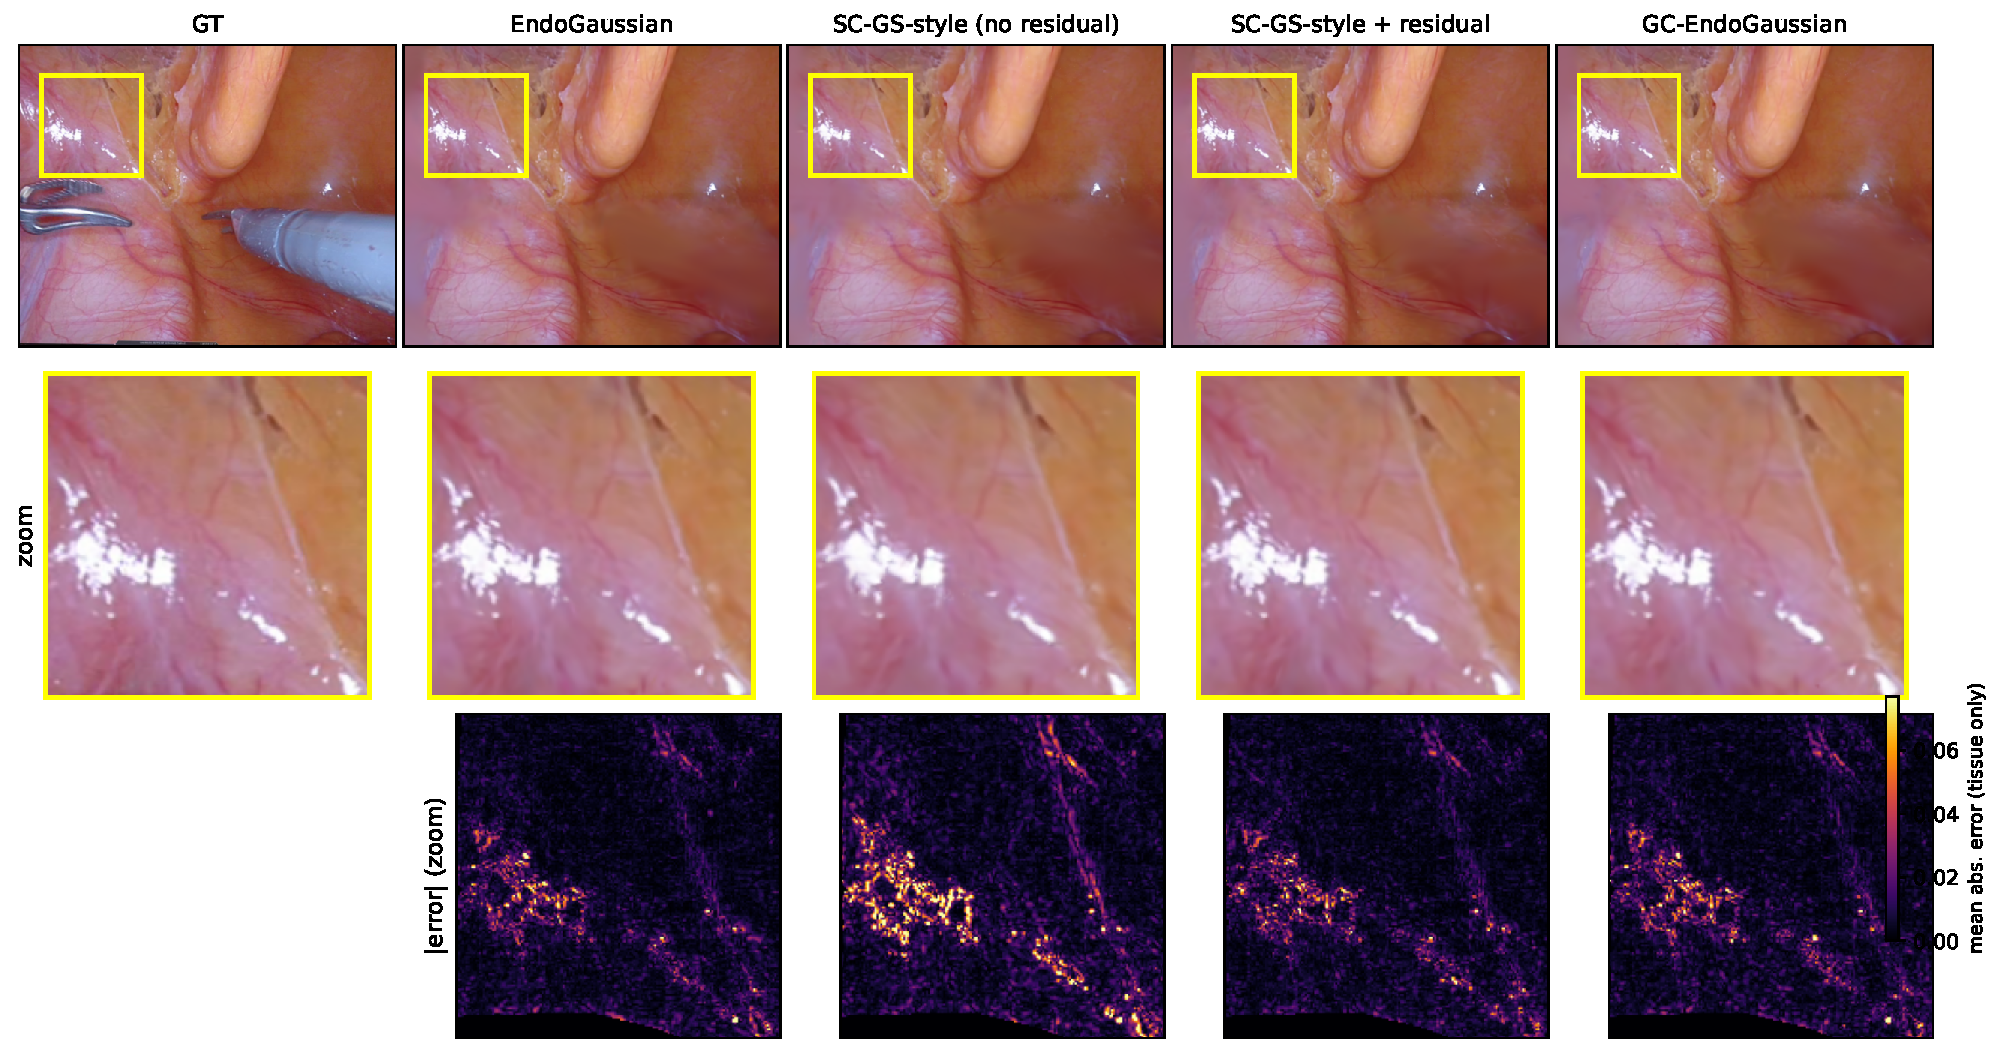
\includegraphics[width=\textwidth]{figures/fig_residual_ablation.pdf}
\caption{What the dense residual fixes. Test frame of \texttt{pulling\_soft\_tissues} (3000 fine-stage iterations, matched budget). Top: rendering with inset location; middle: zoom; bottom: per-pixel error over tissue (tool region excluded from losses and metrics; shared color scale). The SC-GS-style model without the residual (third column) shows visibly higher error on vascular and specular detail; adding the per-Gaussian residual (fourth column) recovers it, matching the $0.52$~dB gap in Table~\ref{tab:residual}.\label{fig:residual_visual}}
\end{figure*}

The central conclusion is therefore architectural but not graph-specific: a sparse-control editor should retain a dense per-Gaussian deformation residual when it is attached to a high-fidelity endoscopic reconstruction model. The result also prevents an incorrect interpretation of the main comparison. GC-EndoGaussian does not outperform every residual-matched sparse-control architecture; rather, it provides one practical configuration that preserves most of the base model's fidelity while exposing explicit controls.

\subsection{Additional ablations and negative results}

Replacing EdgeConv aggregation with GAT-style attention produces no material change in the conclusions, and removing message passing yields similar performance in the residual-matched setting. These observations indicate that graph aggregation is not the main source of reconstruction fidelity.

Additional experiments also show limited benefit from using the graph as a reconstruction prior. Occlusion-holdout performance is similar to the dense field, optical-flow supervision does not improve the reported configuration and becomes harmful at high weight, and an explicit cut-modeling mechanism does not exceed the continuous deformation field at the cut region. These negative results are consistent with the view that the dense HexPlane field already captures smooth observed motion effectively. The sparse graph contributes an editing interface, not additional reconstruction evidence.

\section{Discussion and Limitations}\label{sec6}

GC-EndoGaussian demonstrates that a sparse editing interface can be integrated into an endoscopic 4D Gaussian reconstruction while retaining performance close to a strong dense baseline. The main empirical finding is that the dense per-Gaussian residual is necessary for this outcome. A sparse-control field alone lacks sufficient degrees of freedom to represent local tissue motion at the same fidelity---and, across seeds, it is also less stable to optimize.

The results also clarify what should not be claimed. GC-EndoGaussian does not improve reconstruction quality over EndoGaussian in the main matched comparisons, and the tracking study does not establish statistical equivalence. The contribution is the addition of explicit control with a small reconstruction cost, rather than superior reconstruction or tracking.

The editing mechanism has several limitations:
\begin{itemize}
\item \textbf{Edits are not biomechanically validated.} Node translations generate smooth visual deformations but do not model tissue material properties, force response, cutting mechanics, or anatomical constraints.
\item \textbf{Edit evaluation is geometric, not perceptual.} Section~\ref{sec:edit_eval} quantifies handle fidelity, locality, foldover, and latency, but does not measure the \emph{plausibility} of edited tissue configurations: no user study with surgical experts was conducted, and no comparison against physically simulated deformation is reported.
\item \textbf{Edits bypass graph message passing.} Inference-time translations are added after node-motion prediction. Consequently, the graph does not learn to propagate user input according to tissue behavior. A future model could inject edits before message passing and train the network to distribute them.
\item \textbf{Evaluation breadth is limited.} Reconstruction results cover two EndoNeRF scenes, while tracking uses four SuPer trials from one acquisition setting. Generalization across anatomies, procedures, stereo rigs, and camera motion remains untested.
\item \textbf{Efficiency reporting is incomplete.} Rendering speed, parameter count, and edit-to-render latency are reported, but wall-clock training time and memory use should be measured in a final systems evaluation.
\end{itemize}

These limitations position GC-EndoGaussian as an editable visual reconstruction method and a basis for future interaction research, rather than as a predictive surgical simulator.

\section{Conclusion}\label{sec7}

We introduced GC-EndoGaussian, a sparse control layer for editable endoscopic 4D Gaussian reconstruction. The method binds dense Gaussians to a compact set of control nodes and supports local inference-time edits through weighted node translations, with measured handle fidelity of 0.96, structurally compact edit support, and sub-5~ms edit-to-render latency. A residual-centered integration recipe keeps reconstruction close to EndoGaussian: the PSNR gap is 0.11~dB under the standard schedule averaged over four seeds and 0.13--0.15~dB under the extended schedule, while rendering remains interactive at 205~FPS with 0.07\% additional deformation parameters. The SuPer evaluation detects no significant difference in tracking error from the dense baseline.

The residual-isolation experiment provides the main technical conclusion. An SC-GS-style sparse-control model without a dense residual loses reconstruction and tracking fidelity, leaks edit-induced image change outside the edited region, and fails to converge on some seeds, whereas adding the per-Gaussian residual recovers reconstruction and tracking, confines edits, and stabilizes training. Thus, the key to combining editability with a strong endoscopic reconstruction is not a particular graph aggregator, but the preservation of dense local deformation capacity alongside sparse controls.

Future work should quantify the perceptual plausibility of edits, route user edits through learned message passing, and incorporate biomechanical or anatomical constraints where predictive tissue behavior is required.

% \bmsection*{Author contributions}

% This is an author contribution text. Please replace with the actual contributions of each author.

% \bmsection*{Acknowledgments}

% This is acknowledgment text. Please provide the acknowledgment text here.

% \bmsection*{Financial disclosure}

% None reported.

% \bmsection*{Conflict of interest}

% The authors declare no potential conflict of interests.

\bibliography{wileyNJD-AMA}

%\nocite{*}% Uncomment to show all bib entries (both cited and uncited).

\end{document}
